\chapter{Scopi e Problemi Affrontati}

\section{Applicazioni del MagicMirror}
Il Magic Mirror \`e un software che implementa api, le quali permettono
l'integrazione di applicazioni sviluppate da terzi e forniscono strumenti per la comunicazione, gestione
ed organizzazione tra di esse.
Lo scopo nello sviluppo delle applicazioni, durante lo stage, \`e stato
di creare programmi che permettessero l'interazione tra il software principale
e l'essere umano. Nello specifico si \`e voluto implementare la possibilit\`a, da parte di un utente,
di controllare le applicazioni attive sul Magic Mirror tramite l'impartizione di comandi vocali
o movimenti delle dita su una scheda touchpad.
In questa parte si \`e dovuto affrontare il problema di far comunicare
i diversi dispositivi hardware con il calcolatore principale, e di programmare
le applicazioni con linguaggi diversi, a seconda della compatibilit\`a di un linguaggio
e delle librerie a disposizione di una determinata periferica.
\\[2\baselineskip]
\section{Interfaccia di controllo del MagicMirror}
Nella seconda parte dello stage si \`e svolta la progettazione di un'interfaccia Web di configurazione remota
il cui scopo \`e di permettere ad un utente autenticato di gestire
le configurazioni delle applicazioni implementate nel software da una pagina web,
senza dover accedere fisicamente alla macchina.
Quest'ultima permette anche di disattivare (o attivare) le applicazioni presenti nel Magic Mirror,
la cui procedura, prima, richiedeva di aggiungere manualmente un pezzo di codice nella
configurazione del software princiapale.
Nello sviluppo dell'interfaccia si \`e affrontato il problema di dover modificare
il documento di configurazione del software principale senza eliminarne parti essenziali
o modificarlo in un formato sbagliato.
Lo scambio dei messaggi tra il Magic Mirror e la pagina web avviene in formato JSON, lo stesso formato
usato per il suo file di configurazione e delle sue applicazioni.\\
Un altro problema riscontrato in questa parte è stata la difficoltà dell'utilizzo di Javascript
perchè \`e un linguaggio asincrono, ovvero alcune funzioni venivano eseguite senza attendere
il risulato della precedente. Il linguaggio, per poter sincronizzare la funzioni, mette a disposizione
le callback: funzioni passate come parametro alla funzione principale che a loro volta avevano come paramentro il risultato,
in modo da poter eseguire le operazioni solo dopo che la funzione chiamante avesse prodotto l'output.
Il problema di questo approccio \`e stato il fenomeno "Callback Hell", ovvero Callback che chiamano a loro volta
altre Callback creando funzioni annidate pi\`u volte, come mostrato in figura \ref{fig:hell}.
\\[2\baselineskip]
\begin{figure}[h]
    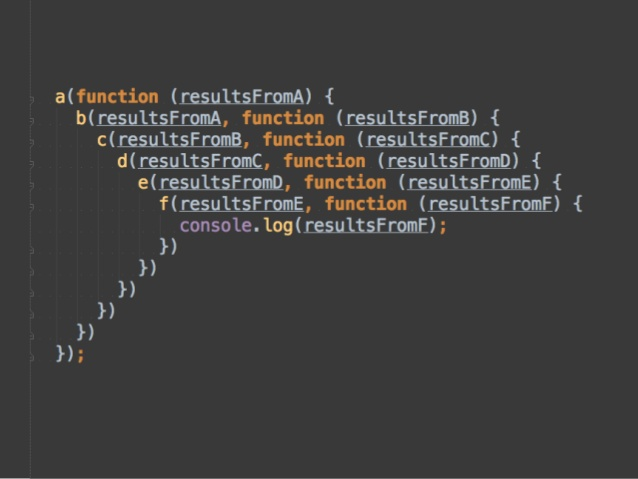
\includegraphics[width=1\textwidth, height=0.4\textheight]{callbackhell}
    \caption{Esempio di Callback Hell}
    \label{fig:hell}
\end{figure}
